\documentclass[12pt,a4paper]{report}

\usepackage[a4paper,margin=1in]{geometry}
\usepackage[T1]{fontenc}
\usepackage{lmodern}
\usepackage{setspace}
\usepackage{graphicx}
\usepackage{array}
\usepackage{amsmath}
\usepackage{booktabs}
\usepackage{longtable}
\usepackage{hyperref}
\usepackage{enumitem}
\usepackage{fancyhdr}
\usepackage{titlesec}
\usepackage{float}
\usepackage{tikz}
\usetikzlibrary{arrows.meta,positioning,shapes.geometric}
\usepackage{xcolor}

\onehalfspacing
\setlength{\parindent}{0pt}
\setlength{\parskip}{6pt}
\hypersetup{colorlinks=true,linkcolor=black,urlcolor=blue,citecolor=black,pdftitle={GovExam Alert Mid-Semester Project Report}}
\pagestyle{fancy}
\fancyhf{}
\fancyhead[L]{UCS503 -- Software Engineering Lab}
\fancyhead[R]{GovExam Alert}
\fancyfoot[C]{\thepage}
\renewcommand{\headrulewidth}{0.4pt}
\setlength{\headheight}{15pt}
\setlist[enumerate]{itemsep=2pt,topsep=3pt}
\setlist[itemize]{itemsep=2pt,topsep=3pt}

\begin{document}

% ---------------- TITLE PAGE ----------------
\begin{titlepage}
\centering
\vspace*{0.7cm}
{\large\textbf{UCS 503 Software Engineering Project Report}\par}
{\large Mid-Semester Evaluation\par}
\vspace{2.0cm}
{\Huge\bfseries Government Exam Notification and Deadline Alert System\par}
\vspace{0.8cm}


\vspace{1.2cm}
{\large\textbf{Submitted by:}\par}
\vspace{0.35cm}
{\large
1024030731 -- Aryan Juneja\\
1024030747 -- Raghav Mittal\\
1024031150 -- Bir Angad\\[0.3cm]
Group: 3C53\\
BE Third Year, COE\par}
\vspace{1.0cm}
{\large\textbf{Submitted to:}\par}
\vspace{0.2cm}
{\large PARAMVEER KAUR\par}
\vfill
{\large Computer Science and Engineering Department\par}
{\large Thapar Institute of Engineering and Technology, Patiala\par}
\vspace{0.4cm}
{\large Submission Date: 16 October 2026\par}
\end{titlepage}

\pagenumbering{roman}
\tableofcontents
\clearpage
\pagenumbering{arabic}

% ---------------- CHAPTER 1 ----------------
\chapter{Introduction}

\section{Background and Context}
Government recruitment examinations are announced by multiple organisations, each publishing information such as eligibility, application dates, examination dates, and official application links. Aspirants often need to visit several websites and manually track deadlines. This can make it difficult to compare opportunities and may cause applicants to miss important dates.

GovExam Alert is a web-based project intended to organise government examination information in one accessible portal. Its interface presents exam details in a structured form, while a backend API is being developed to retrieve and manage exam records. Deadline reminders and complete persistent data integration are planned extensions of the current prototype.

\subsection{Problem Statement}
Exam-related information is spread across multiple official sources and may be updated at different times. Users need a straightforward way to find relevant examinations and review their key dates and application links. The project addresses this need through a centralised listing interface and a planned data-management workflow. Official notifications remain the authoritative source for dates, eligibility, and application instructions.

\section{Project Objectives}
The objectives of the project are:
\begin{enumerate}[label=\arabic*.]
  \item Build a clear web interface that displays government examination listings and their key details.
  \item Develop backend API routes to retrieve exam records and support administrative creation, updating, and deletion.
  \item Connect the frontend to backend data and verify that records can be stored and retrieved reliably.
  \item Plan and implement deadline reminders after the core data flow is stable.
  \item Test the system's main user flows and API operations, documenting observed results and unresolved issues.
\end{enumerate}

This report documents the work completed so far and clearly identifies unfinished items. The frontend prototype and parts of the exam-management API have been developed, but backend reliability, complete frontend--backend integration, database persistence verification, and deadline-reminder delivery remain unfinished or require retesting. The design models show the intended project behaviour; they do not mean that every feature is operational.

\section{Project Scope}
The current scope focuses on displaying exam information and building a basic API for exam records. The wider intended scope includes persistent data management, search and category filtering, administrative exam management, and deadline reminders. The project is an academic prototype and should not be treated as an official source of recruitment information or as a production-ready notification service.

% ---------------- CHAPTER 2 ----------------
\chapter{Methodology and Design}

\section{System Architecture}
GovExam Alert is intended to use a client--server design. The React frontend presents exam listings and user interactions; the Express backend exposes routes for reading and managing exam records; and SQLite is the planned local data store. These parts are not yet verified as a reliable end-to-end integration. The evaluation chapter records the tests actually observed and identifies unfinished integration and data-persistence checks.

\subsection{High-Level Design}
Figure~\ref{fig:architecture} presents the intended components. The reminder component is planned and the end-to-end connections still require verification.

\begin{figure}[H]
\centering
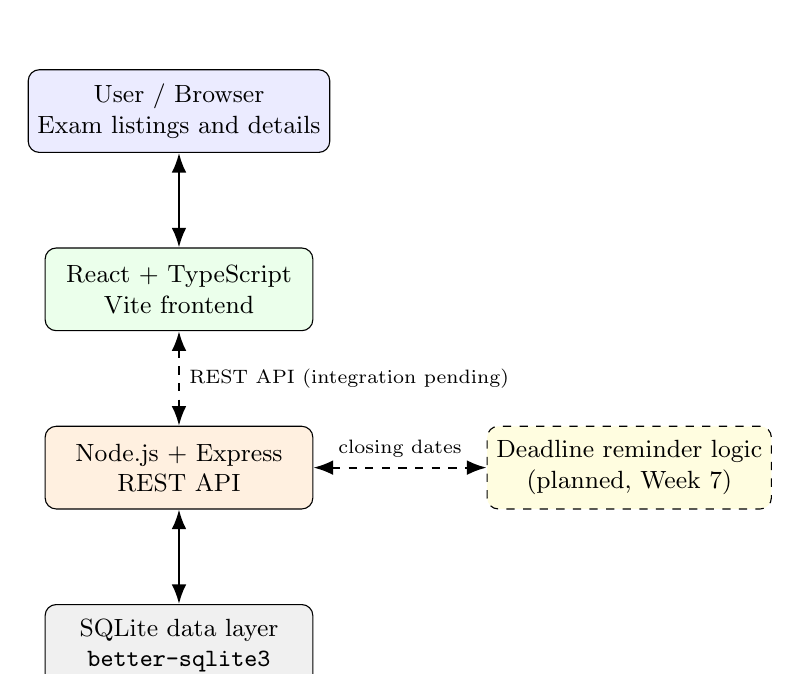
\begin{tikzpicture}[
  node distance=1.2cm and 1.3cm,
  comp/.style={draw,rounded corners,align=center,minimum width=3.4cm,minimum height=1.05cm,font=\small},
  planned/.style={draw,dashed,rounded corners,align=center,minimum width=3.4cm,minimum height=1.05cm,font=\small},
  arr/.style={{Latex[length=2.5mm]}-{Latex[length=2.5mm]},thick},
  parr/.style={{Latex[length=2.5mm]}-{Latex[length=2.5mm]},thick,dashed}
]
\node[comp,fill=blue!8] (user) {User / Browser\\Exam listings and details};
\node[comp,fill=green!8,below=of user] (front) {React + TypeScript\\Vite frontend};
\node[comp,fill=orange!12,below=of front] (api) {Node.js + Express\\REST API};
\node[comp,fill=gray!12,below=of api] (db) {SQLite data layer\\\texttt{better-sqlite3}};
\node[planned,fill=yellow!12,right=2.2cm of api] (rem) {Deadline reminder logic\\(planned, Week 7)};
\draw[arr] (user) -- (front);
\draw[parr] (front) -- node[right,font=\scriptsize]{REST API (integration pending)} (api);
\draw[arr] (api) -- (db);
\draw[parr] (api) -- node[above,font=\scriptsize]{closing dates} (rem);
\end{tikzpicture}
\caption{High-level architecture of GovExam Alert. Dashed elements and links indicate planned or not-yet-verified functionality.}
\label{fig:architecture}
\end{figure}

\subsection{Technical Stack}
\begin{longtable}{p{0.28\textwidth} p{0.62\textwidth}}
\toprule
\textbf{Component} & \textbf{Technology / Tool}\\
\midrule
Frontend & React with TypeScript\\
Build and development server & Vite\\
Routing and icons & React Router and Lucide React\\
Backend & Node.js and Express\\
Database layer & SQLite with \texttt{better-sqlite3}\\
API testing & Thunder Client\\
Development environment & Visual Studio Code and npm\\
Version control & Git and GitHub\\
\bottomrule
\end{longtable}

\section{Implementation Details}
\subsection{Module 1: Exam Listing Interface}
The frontend prototype includes a landing page for GovExam Alert and exam cards. The exam data model contains fields such as exam title, recruiting organisation, category, application last date, exam date, application link, description, eligibility information, number of posts, and an indicator for new listings. Sample records include SSC CGL, UPSC Civil Services, and other illustrative examination entries in the frontend prototype.

The frontend currently demonstrates the presentation and browsing experience. Because some screens use mock data, the visible listings should not be interpreted as proof that every record is being loaded from the backend or verified against a live official notification.

\subsection{Module 2: Backend API and Data Management}
The Express backend exposes a basic health route and exam-related endpoints, including routes to retrieve exam records and administrative routes for creating, updating, and deleting records. Search and category-filtering functionality is part of the API work. SQLite with \texttt{better-sqlite3} has been installed for local data storage.

Previously recorded Thunder Client tests showed a successful POST response with HTTP status 201 and a successful PUT response with HTTP status 200. A DELETE request returned HTTP 404 during testing and remains unresolved. At the latest reporting point, backend API response-time measurements have not been collected because the API is not currently working reliably. These operations must be retested after the issue is fixed.

\subsection{Planned Module: Deadline Reminders}
The Week 7 design includes a deadline-reminder workflow based on application closing dates. Reminder intervals, delivery channels, scheduling logic, and user preferences should be validated against the final implementation before the feature is considered operational.

\section{Analysis Phase: Requirements and Models}
This section expands the design documentation using the analysis deliverables represented in the two reference reports. The diagrams model the intended GovExam Alert workflow; they do not imply that every depicted feature has already been implemented. In particular, reminders and complete frontend--backend integration remain planned work.

\subsection{Actors and Use-Case Diagram}
The primary actor is the aspirant/user who browses exam listings, searches by category or keyword, views details and follows official application links. An administrator maintains examination records through create, update and delete operations. The backend API and database support these interactions. Deadline reminders are a planned use case.

\begin{figure}[H]
\centering
\resizebox{\textwidth}{!}{%
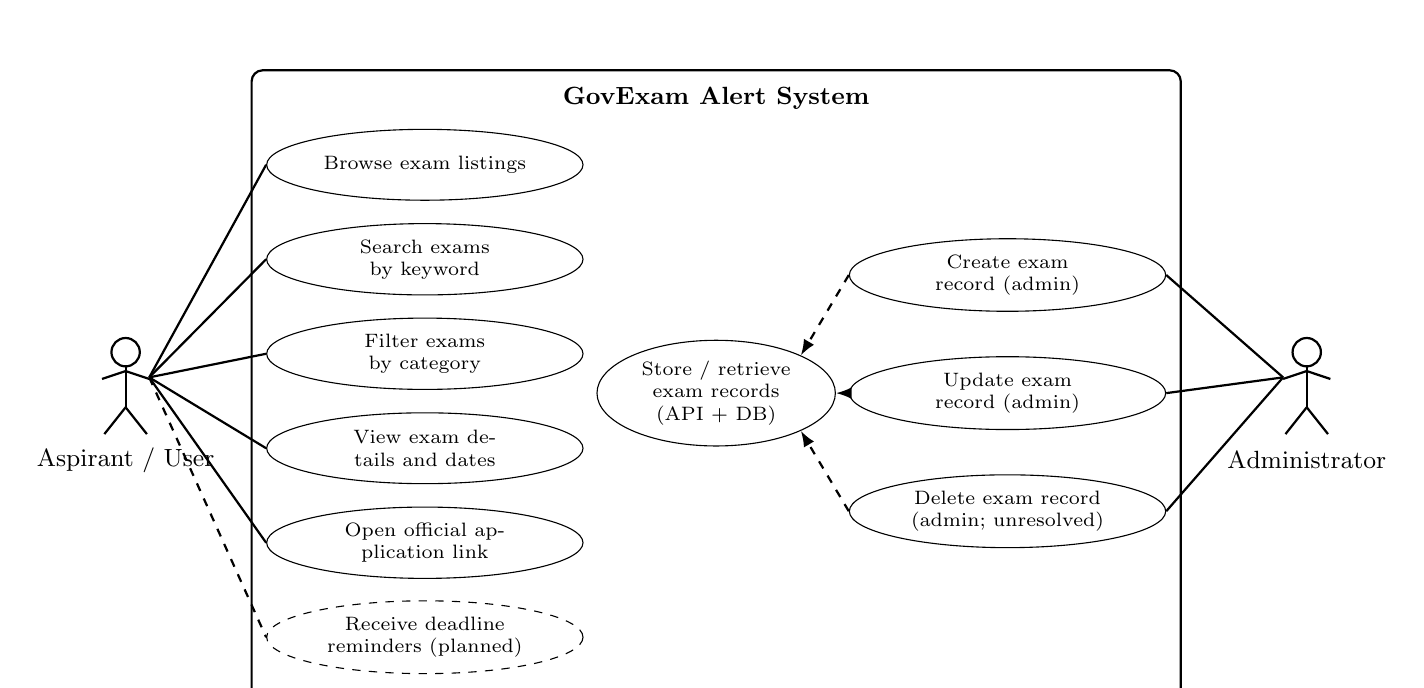
\begin{tikzpicture}[
  x=1cm,y=1cm,
  uc/.style={draw,ellipse,align=center,text width=2.7cm,minimum height=.9cm,font=\scriptsize,inner sep=2pt},
  planned/.style={uc,dashed},
  inc/.style={-{Latex[length=2mm]},dashed,thick}
]
% ---- Actor: Aspirant ----
\draw[thick] (0,0.52) circle (0.18);
\draw[thick] (0,0.34) -- (0,-0.18);
\draw[thick] (-0.30,0.18) -- (0,0.28) -- (0.30,0.18);
\draw[thick] (0,-0.18) -- (-0.27,-0.52);
\draw[thick] (0,-0.18) -- (0.27,-0.52);
\node[font=\small] at (0,-0.85) {Aspirant / User};
% ---- Actor: Administrator ----
\draw[thick] (15,0.52) circle (0.18);
\draw[thick] (15,0.34) -- (15,-0.18);
\draw[thick] (14.70,0.18) -- (15,0.28) -- (15.30,0.18);
\draw[thick] (15,-0.18) -- (14.73,-0.52);
\draw[thick] (15,-0.18) -- (15.27,-0.52);
\node[font=\small] at (15,-0.85) {Administrator};
% ---- System boundary ----
\draw[rounded corners,thick] (1.6,-3.9) rectangle (13.4,4.1);
\node[font=\small\bfseries] at (7.5,3.75) {GovExam Alert System};
% ---- User use cases (one column, so no line crosses another ellipse) ----
\node[uc] (browse)   at (3.8, 2.9) {Browse exam listings};
\node[uc] (search)   at (3.8, 1.7) {Search exams by keyword};
\node[uc] (filter)   at (3.8, 0.5) {Filter exams by category};
\node[uc] (details)  at (3.8,-0.7) {View exam details and dates};
\node[uc] (official) at (3.8,-1.9) {Open official application link};
\node[planned] (reminder) at (3.8,-3.1) {Receive deadline reminders (planned)};
% ---- Admin use cases ----
\node[uc] (create) at (11.2, 1.5) {Create exam record (admin)};
\node[uc] (update) at (11.2, 0.0) {Update exam record (admin)};
\node[uc] (delete) at (11.2,-1.5) {Delete exam record (admin; unresolved)};
% ---- Shared system use case ----
\node[uc,text width=2.0cm] (retrieve) at (7.5,0) {Store / retrieve exam records (API + DB)};
% ---- Associations ----
\foreach \n in {browse,search,filter,details,official}{\draw[thick] (0.3,0.2) -- (\n.west);}
\draw[thick,dashed] (0.3,0.2) -- (reminder.west);
\foreach \n in {create,update,delete}{\draw[thick] (14.7,0.2) -- (\n.east);}
% ---- <<include>> ----
\draw[inc] (create.west) -- (retrieve.north east);
\draw[inc] (update.west) -- (retrieve.east);
\draw[inc] (delete.west) -- (retrieve.south east);
\end{tikzpicture}%
}
\caption{Use-case diagram for GovExam Alert. Dashed ellipse = planned feature; dashed arrows = \guillemotleft include\guillemotright{} relationships. The delete operation has a recorded HTTP 404 failure.}
\label{fig:usecase}
\end{figure}

\subsection{Use-Case Templates}
\textbf{UC-01: Browse Exam Listings}\par
\textbf{Actor:} Aspirant/user. \textbf{Precondition:} The application is open.\par
\textbf{Main flow:} (1) User opens the listing page. (2) The system displays available exam cards. (3) User browses the cards and selects an exam. (4) The system displays available details.\par
\textbf{Alternative flow:} If no records are available, the interface should show an empty state or an error message.\par
\textbf{Postcondition:} The user can view the available exam information.

\textbf{UC-02: Search or Filter Exams}\par
\textbf{Actor:} Aspirant/user. \textbf{Precondition:} Exam listings are available.\par
\textbf{Main flow:} (1) User enters a keyword or selects a category. (2) The system applies the search/filter condition. (3) Matching records are displayed.\par
\textbf{Alternative flow:} If there are no matches, show a clear no-results message.\par
\textbf{Postcondition:} A filtered list or a no-results state is displayed.

\textbf{UC-03: Manage Exam Record}\par
\textbf{Actor:} Administrator. \textbf{Precondition:} The admin endpoint is available and the request contains a valid record.\par
\textbf{Main flow:} (1) Admin submits a create or update request. (2) API validates the request. (3) The record is stored or updated. (4) API returns a success response.\par
\textbf{Alternative flow:} Invalid data or a missing record returns an appropriate error. Delete behaviour requires further testing because a recorded DELETE request returned HTTP 404.\par
\textbf{Postcondition:} The operation result is returned; persistence must be verified through regression tests.

\textbf{UC-04: Follow Official Application Link}\par
\textbf{Actor:} Aspirant/user. \textbf{Precondition:} An exam record includes an application URL.\par
\textbf{Main flow:} User opens exam details and selects the official application link; the browser navigates to the supplied destination.\par
\textbf{Alternative flow:} If the URL is missing or unavailable, the interface should tell the user to consult the recruiting organisation's official website.\par
\textbf{Postcondition:} User is directed to the provided official source.

\textbf{UC-05: Receive Deadline Reminder (Planned)}\par
\textbf{Actor:} Aspirant/user; supporting component: reminder scheduler. \textbf{Precondition:} Reminder logic and delivery method have been implemented and configured.\par
\textbf{Main flow:} The scheduler checks upcoming closing dates and sends reminders according to configured intervals.\par
\textbf{Alternative flow:} Missing dates or failed delivery are logged and must not be represented as a successful reminder.\par
\textbf{Postcondition:} A reminder is delivered only when the planned service is operational. This use case belongs to the Week 7 scope; successful delivery still requires verification.

\subsection{Activity Diagram}
Figure~\ref{fig:activity} describes the user browsing flow and the planned reminder branch.
\begin{figure}[H]\centering
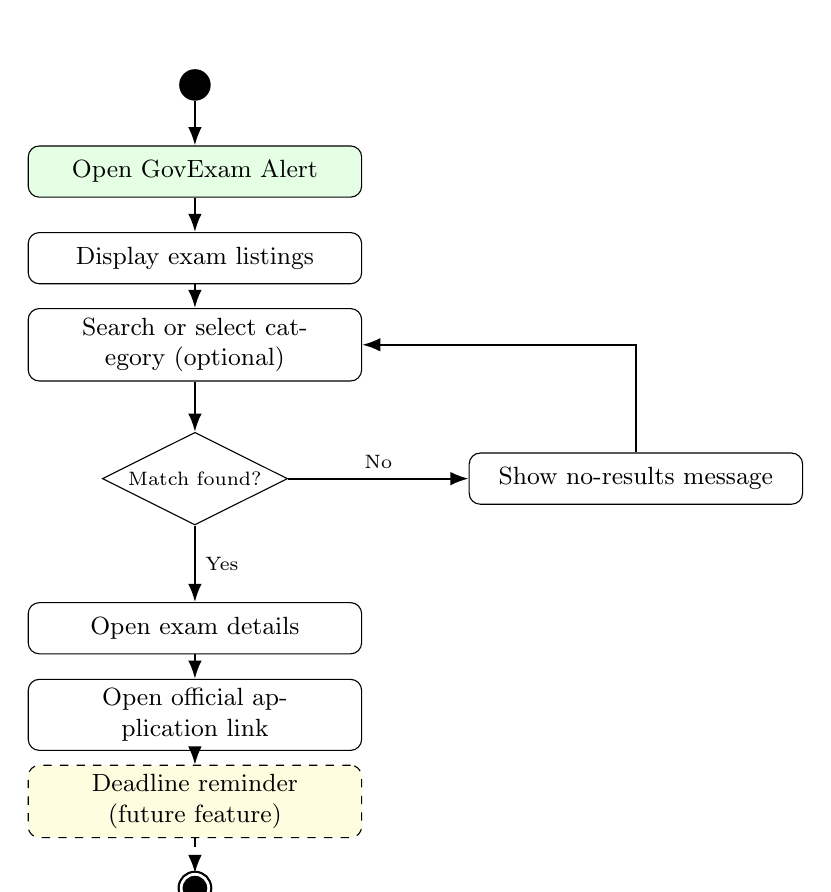
\begin{tikzpicture}[
  act/.style={draw,rounded corners,align=center,text width=4.0cm,minimum height=.65cm,font=\small},
  dec/.style={draw,diamond,aspect=2,align=center,text width=1.8cm,inner sep=1pt,font=\scriptsize},
  ini/.style={circle,fill=black,minimum size=.4cm,inner sep=0pt},
  fin/.style={circle,draw,thick,double,double distance=1pt,fill=black,minimum size=.35cm,inner sep=0pt},
  arr/.style={-Latex,thick}
]
\node[ini] (start) at (0,0) {};
\node[act,fill=green!10] (open)   at (0,-1.1) {Open GovExam Alert};
\node[act] (list)   at (0,-2.2) {Display exam listings};
\node[act] (filter) at (0,-3.3) {Search or select category (optional)};
\node[dec] (found)  at (0,-5.0) {Match found?};
\node[act] (empty)  at (5.6,-5.0) {Show no-results message};
\node[act] (details) at (0,-6.9) {Open exam details};
\node[act] (official) at (0,-8.0) {Open official application link};
\node[act,fill=yellow!12,dashed] (rem) at (0,-9.1) {Deadline reminder (future feature)};
\node[fin] (end) at (0,-10.2) {};
\draw[arr] (start)--(open);
\draw[arr] (open)--(list);
\draw[arr] (list)--(filter);
\draw[arr] (filter)--(found);
\draw[arr] (found)--node[above,font=\scriptsize]{No}(empty);
\draw[arr] (found)--node[right,font=\scriptsize]{Yes}(details);
\draw[arr] (empty.north) |- (filter.east);   % loop back to search again
\draw[arr] (details)--(official);
\draw[arr,dashed] (official)--(rem);
\draw[arr,dashed] (rem)--(end);
\end{tikzpicture}
\caption{Activity diagram of the user browsing workflow. The no-results branch returns to search; the reminder step is planned.}\label{fig:activity}
\end{figure}

\subsection{Swimlane Workflow}
\begin{figure}[H]\centering
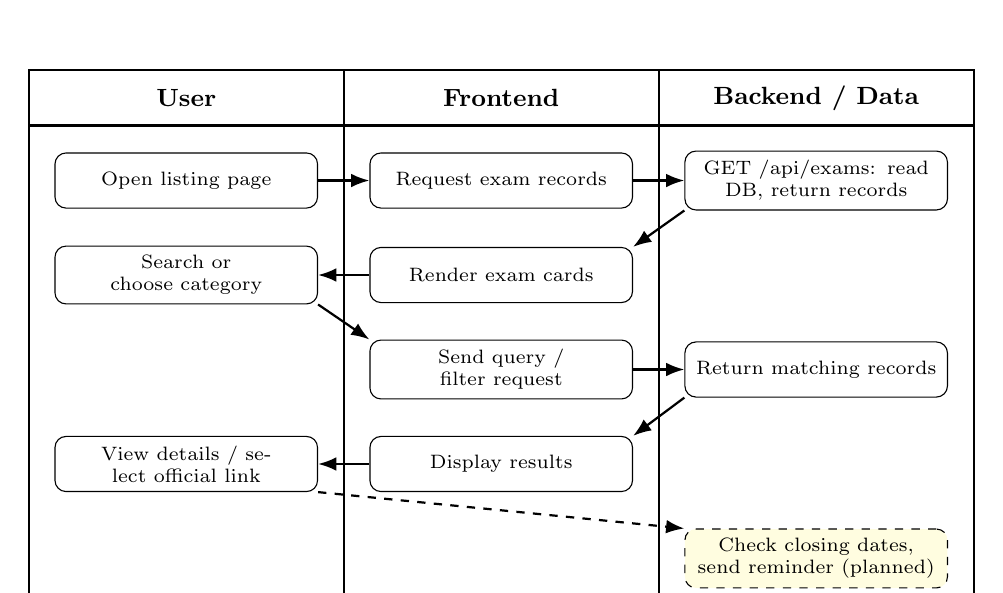
\begin{tikzpicture}[x=1cm,y=1cm,
  stepbox/.style={draw,rounded corners,align=center,text width=3.1cm,minimum height=.7cm,font=\scriptsize},
  arr/.style={-Latex,thick}]
\draw[thick] (0,-1.1) rectangle (12,5.7);
\draw[thick] (4,-1.1)--(4,5.7);
\draw[thick] (8,-1.1)--(8,5.7);
\draw[thick] (0,5.0)--(12,5.0);
\node[font=\small\bfseries] at (2,5.35)  {User};
\node[font=\small\bfseries] at (6,5.35)  {Frontend};
\node[font=\small\bfseries] at (10,5.35) {Backend / Data};

\node[stepbox] (u1) at (2,4.3)  {Open listing page};
\node[stepbox] (f1) at (6,4.3)  {Request exam records};
\node[stepbox] (b1) at (10,4.3) {GET /api/exams: read DB, return records};

\node[stepbox] (u2) at (2,3.1)  {Search or choose category};
\node[stepbox] (f2) at (6,3.1)  {Render exam cards};

\node[stepbox] (f3) at (6,1.9)  {Send query / filter request};
\node[stepbox] (b2) at (10,1.9) {Return matching records};

\node[stepbox] (u3) at (2,0.7)  {View details / select official link};
\node[stepbox] (f4) at (6,0.7)  {Display results};

\node[stepbox,fill=yellow!12,dashed] (b3) at (10,-0.5) {Check closing dates, send reminder (planned)};

\draw[arr] (u1)--(f1);
\draw[arr] (f1)--(b1);
\draw[arr] (b1.south west)--(f2.north east);
\draw[arr] (f2)--(u2);
\draw[arr] (u2.south east)--(f3.north west);
\draw[arr] (f3)--(b2);
\draw[arr] (b2.south west)--(f4.north east);
\draw[arr] (f4)--(u3);
\draw[arr,dashed] (u3.south east)--(b3.north west);
\end{tikzpicture}
\caption{Swimlane view of the user, frontend, and backend responsibilities. All backend data reaches the user through the frontend.}\label{fig:swimlane}
\end{figure}

\subsection{Data Flow Diagrams}
\subsubsection{DFD Level 0: Context Diagram}
\begin{figure}[H]\centering
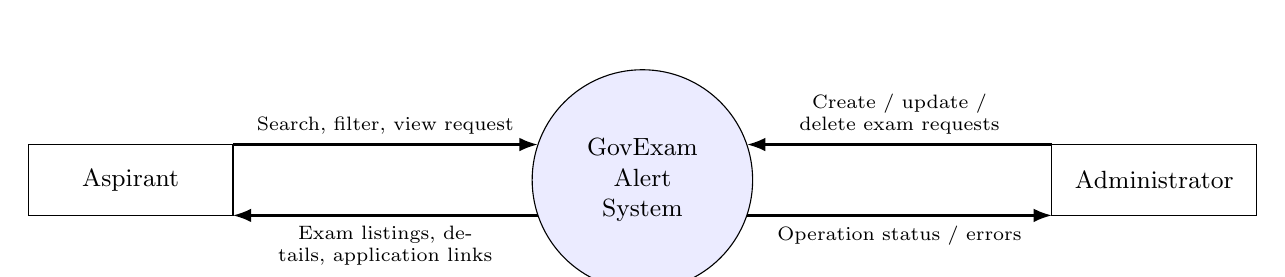
\begin{tikzpicture}[
  ent/.style={draw,rectangle,align=center,minimum width=2.6cm,minimum height=.9cm,font=\small},
  proc/.style={draw,circle,align=center,minimum size=2.8cm,font=\small},
  arr/.style={-Latex,thick},
  lab/.style={font=\scriptsize,align=center,text width=3.6cm}]
\node[ent] (user)  at (0,0)    {Aspirant};
\node[proc,fill=blue!8] (sys) at (6.5,0) {GovExam\\Alert\\System};
\node[ent] (admin) at (13,0)   {Administrator};
% two separate parallel arrows per pair (no overlap)
\draw[arr] (1.3,0.45)--node[above,lab]{Search, filter, view request}(5.17,0.45);
\draw[arr] (5.17,-0.45)--node[below,lab]{Exam listings, details, application links}(1.3,-0.45);
\draw[arr] (11.7,0.45)--node[above,lab]{Create / update / delete exam requests}(7.83,0.45);
\draw[arr] (7.83,-0.45)--node[below,lab]{Operation status / errors}(11.7,-0.45);
\end{tikzpicture}
\caption{DFD Level 0 showing external actors and the system boundary.}\label{fig:dfd0}
\end{figure}

\subsubsection{DFD Level 1: Main Processes}
\begin{figure}[H]\centering
\resizebox{\textwidth}{!}{%
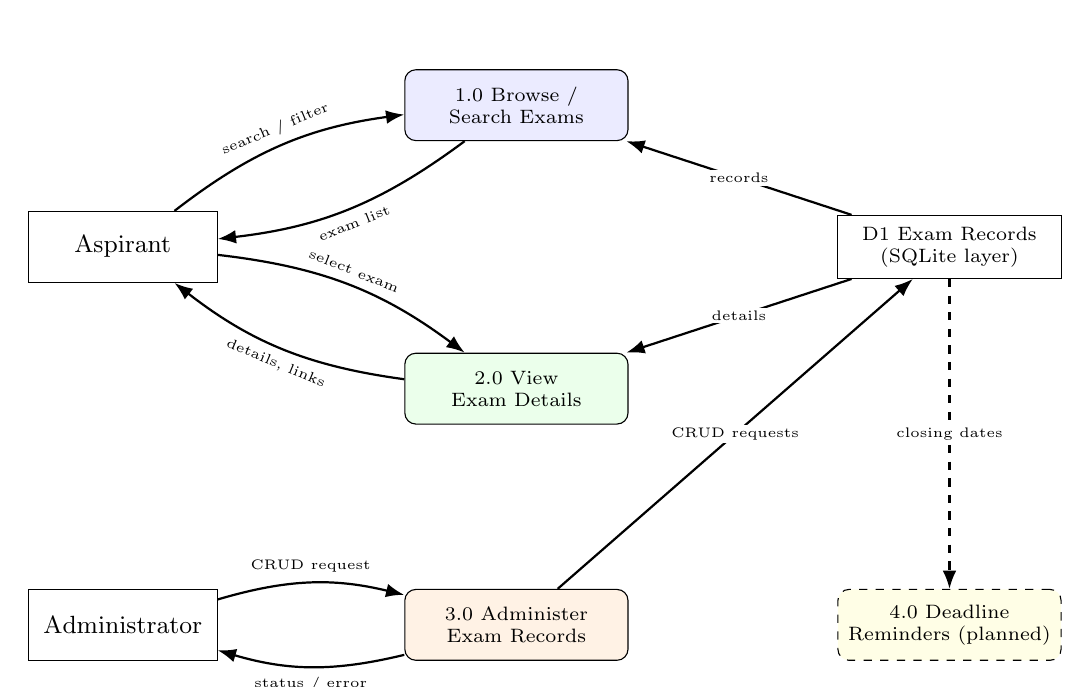
\begin{tikzpicture}[
  ent/.style={draw,rectangle,align=center,minimum width=2.4cm,minimum height=.9cm,font=\small},
  p/.style={draw,rounded corners,align=center,text width=2.6cm,minimum height=.9cm,font=\scriptsize},
  d/.style={draw,align=center,text width=2.6cm,minimum height=.8cm,font=\scriptsize},
  arr/.style={-Latex,thick},
  lb/.style={font=\tiny,fill=white,inner sep=1pt,midway}]
\node[ent] (asp) at (0,2.2) {Aspirant};
\node[p,fill=blue!8]  (p1) at (5,4.0)  {1.0 Browse / Search Exams};
\node[p,fill=green!8] (p2) at (5,0.4)  {2.0 View Exam Details};
\node[d] (d1) at (10.5,2.2) {D1 Exam Records (SQLite layer)};
\node[ent] (adm) at (0,-2.6) {Administrator};
\node[p,fill=orange!10] (p3) at (5,-2.6) {3.0 Administer Exam Records};
\node[p,dashed,fill=yellow!10] (p4) at (10.5,-2.6) {4.0 Deadline Reminders (planned)};

\draw[arr] (asp) to[bend left=15] node[above,sloped,font=\tiny]{search / filter} (p1);
\draw[arr] (p1) to[bend left=15] node[below,sloped,font=\tiny]{exam list} (asp);
\draw[arr] (asp) to[bend left=15] node[above,sloped,font=\tiny]{select exam} (p2);
\draw[arr] (p2) to[bend left=15] node[below,sloped,font=\tiny]{details, links} (asp);

\draw[arr] (d1) -- node[lb]{records} (p1);
\draw[arr] (d1) -- node[lb]{details} (p2);

\draw[arr] (adm) to[bend left=15] node[above,font=\tiny]{CRUD request} (p3);
\draw[arr] (p3) to[bend left=15] node[below,font=\tiny]{status / error} (adm);
\draw[arr] (p3) -- node[lb]{CRUD requests} (d1);

\draw[arr,dashed] (d1) -- node[lb]{closing dates} (p4);
\end{tikzpicture}%
}
\caption{DFD Level 1 showing external entities, browsing, details, administration, and the planned reminder process.}\label{fig:dfd1}
\end{figure}

\subsubsection{DFD Level 2: Exam Administration}
\begin{figure}[H]\centering
\resizebox{\textwidth}{!}{%
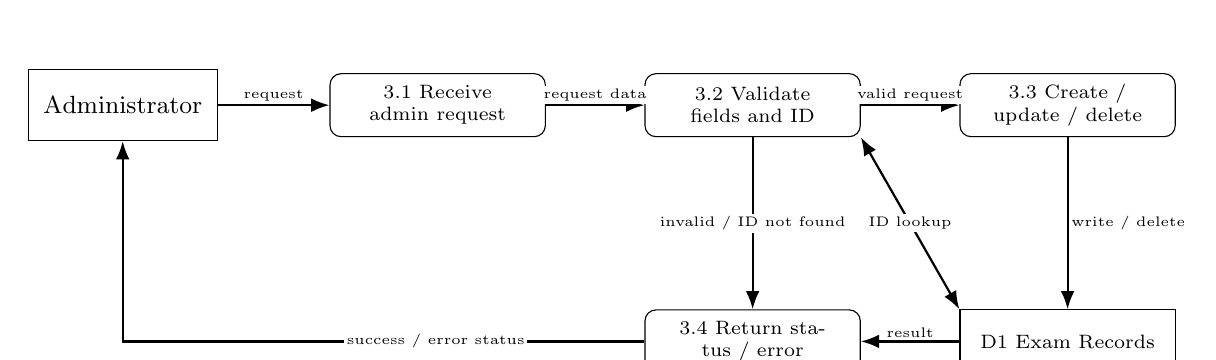
\begin{tikzpicture}[
  ent/.style={draw,rectangle,align=center,minimum width=2.4cm,minimum height=.9cm,font=\small},
  p/.style={draw,rounded corners,align=center,text width=2.5cm,minimum height=.8cm,font=\scriptsize},
  d/.style={draw,align=center,text width=2.5cm,minimum height=.8cm,font=\scriptsize},
  arr/.style={-Latex,thick},
  lb/.style={font=\tiny,fill=white,inner sep=1pt,align=center}]
\node[ent] (adm) at (0,2.2) {Administrator};
\node[p] (p1) at (4,2.2)  {3.1 Receive admin request};
\node[p] (p2) at (8,2.2)  {3.2 Validate fields and ID};
\node[p] (p3) at (12,2.2) {3.3 Create / update / delete};
\node[p] (p4) at (8,-0.8) {3.4 Return status / error};
\node[d] (st) at (12,-0.8) {D1 Exam Records};

\draw[arr] (adm)--node[above,lb]{request}(p1);
\draw[arr] (p1)--node[above,lb]{request data}(p2);
\draw[arr] (p2)--node[above,lb]{valid request}(p3);
\draw[arr] (p3)--node[right,lb]{write / delete}(st);
\draw[arr] (st)--node[above,lb]{result}(p4);
\draw[arr] (p2)--node[lb,midway]{invalid / ID not found}(p4);
\draw[Latex-Latex,thick] (p2.south east)--node[lb,midway]{ID lookup}(st.north west);
\draw[arr] (p4.west) -| node[lb,pos=0.2]{success / error status} (adm.south);
\end{tikzpicture}%
}
\caption{DFD Level 2 expanding administrative exam-record processing, including the ID existence check against the data store.}\label{fig:dfd2}
\end{figure}

\subsection{Sequence Diagram}
\begin{figure}[H]\centering
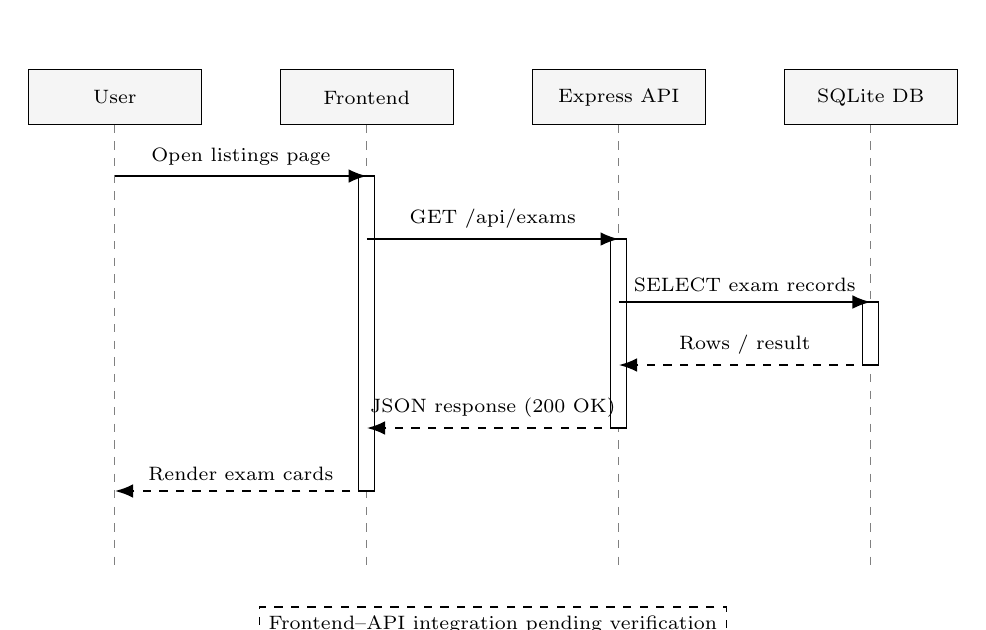
\begin{tikzpicture}[
  life/.style={draw,minimum width=2.2cm,minimum height=.7cm,align=center,font=\scriptsize,fill=gray!8},
  msg/.style={-Latex,thick},
  ret/.style={-Latex,thick,dashed}]
\node[life] at (0,4.2)   {User};
\node[life] at (3.2,4.2) {Frontend};
\node[life] at (6.4,4.2) {Express API};
\node[life] at (9.6,4.2) {SQLite DB};
\foreach \x in {0,3.2,6.4,9.6} {\draw[dashed,gray] (\x,3.85)--(\x,-1.8);}
% activation bars
\draw[fill=white] (3.1,-0.8) rectangle (3.3,3.2);
\draw[fill=white] (6.3,0.0)  rectangle (6.5,2.4);
\draw[fill=white] (9.5,0.8)  rectangle (9.7,1.6);
% messages
\draw[msg] (0,3.2)--node[above,font=\scriptsize]{Open listings page}(3.2,3.2);
\draw[msg] (3.2,2.4)--node[above,font=\scriptsize]{GET /api/exams}(6.4,2.4);
\draw[msg] (6.4,1.6)--node[above,font=\scriptsize]{SELECT exam records}(9.6,1.6);
\draw[ret] (9.6,0.8)--node[above,font=\scriptsize]{Rows / result}(6.4,0.8);
\draw[ret] (6.4,0.0)--node[above,font=\scriptsize]{JSON response (200 OK)}(3.2,0.0);
\draw[ret] (3.2,-0.8)--node[above,font=\scriptsize]{Render exam cards}(0,-0.8);
\node[draw,dashed,font=\scriptsize,align=center] at (4.8,-2.5) {Frontend--API integration pending verification};
\end{tikzpicture}
\caption{Intended sequence for retrieving exam listings (solid = request, dashed = response); current frontend integration remains pending.}\label{fig:sequence}
\end{figure}

\subsection{Data Model}
The planned core exam record contains an identifier, title, recruiting organisation, category, application closing date, exam date, official application URL, description, eligibility details, and number of posts. Additional fields may be added only when needed and supported by the source notification. Database persistence and frontend consumption must be verified through testing.

\section{Software Requirements Specification (IEEE-Style)}
This concise SRS follows an IEEE-style organisation for a course project. It documents intended requirements and is not a claim that all requirements are implemented.

\subsection{Purpose and Scope}
GovExam Alert aims to help aspirants browse government exam information in one portal. The baseline scope includes listing exam records, viewing details, searching/filtering records, and maintaining records through administrative API operations. Reminder delivery is a planned extension.

\subsection{User Classes and Operating Environment}
\begin{itemize}
\item \textbf{Aspirant/user:} browses, searches, filters, views details and follows official application links.
\item \textbf{Administrator:} creates, updates and deletes exam records through administrative endpoints.
\item \textbf{Operating environment:} modern desktop browser; React/TypeScript frontend; Node.js/Express backend; local SQLite data layer.
\end{itemize}

\subsection{Functional Requirements}
\begin{longtable}{p{0.15\textwidth} p{0.76\textwidth}}
\toprule\textbf{ID} & \textbf{Requirement}\\\midrule
FR-01 & The system shall display a list of available examination records.\\
FR-02 & The system shall display key exam details, including title, organisation, category, dates, description and application link when available.\\
FR-03 & The system shall support searching or filtering examination records where the corresponding endpoint/interface is available.\\
FR-04 & The system shall provide an official application URL when one is recorded.\\
FR-05 & The backend shall expose an endpoint to retrieve examination records.\\
FR-06 & The backend shall support creating a valid exam record through an administrative endpoint.\\
FR-07 & The backend shall support updating an existing exam record through an administrative endpoint.\\
FR-08 & The backend shall support deleting an exam record; the recorded DELETE failure must be fixed and retested.\\
FR-09 & The system shall validate required fields and return clear success or error responses.\\
FR-10 & The system should provide deadline reminders once scheduling and delivery are implemented.\\
\bottomrule
\caption{Functional requirements for GovExam Alert.}\label{tab:fr}
\end{longtable}

\subsection{Non-Functional Requirements}
\begin{longtable}{p{0.15\textwidth} p{0.76\textwidth}}
\toprule\textbf{ID} & \textbf{Requirement}\\\midrule
NFR-01 & Usability: exam information should be organised into readable cards or detail views.\\
NFR-02 & Reliability: API errors should be reported clearly and should not silently appear as valid data.\\
NFR-03 & Data integrity: required exam fields and record identifiers should be validated.\\
NFR-04 & Maintainability: frontend presentation, API logic and data access should remain separated.\\
NFR-05 & Performance: page and API response times should be measured under documented conditions; no API target is claimed as achieved yet.\\
NFR-06 & Accuracy: dates, eligibility and URLs should be checked against official recruiting notifications before being presented as verified current information.\\
NFR-07 & Compatibility: the frontend should operate in a current mainstream browser.\\
\bottomrule
\caption{Non-functional requirements.}\label{tab:nfr}
\end{longtable}

\subsection{Data Requirements and Constraints}
An exam record should contain an ID, title, organisation, category, last application date, exam date, official application link and description where available. Eligibility and number of posts may be included when available in the source. Dates and application details can change; official recruiting notifications remain authoritative. The backend's current DELETE failure and incomplete frontend integration are known implementation constraints.

\subsection{Assumptions and Dependencies}
\begin{itemize}
\item Users have access to a modern browser and an internet connection or the local development environment.
\item Official recruitment organisations publish the authoritative exam details.
\item Backend routes and database connectivity must be available for live data to be displayed.
\item Reminder functionality depends on a reliable source of closing dates and a configured delivery/scheduling mechanism.
\end{itemize}

\section{User Stories and Story Cards}
User stories state the expected value from the user's perspective. Acceptance criteria are proposed verification conditions; they do not indicate that a feature has passed testing.

\begin{longtable}{p{0.10\textwidth} p{0.25\textwidth} p{0.38\textwidth} p{0.15\textwidth}}
\toprule\textbf{ID} & \textbf{Story} & \textbf{Acceptance criteria} & \textbf{Priority}\\\midrule
US-01 & As an aspirant, I want to browse exam listings so that I can discover opportunities. & Listings display available exam titles and basic details; empty/error states are clear. & High\\
US-02 & As an aspirant, I want to search or filter exams so that I can narrow results. & Query/category filters return matching records and show a no-results state. & High\\
US-03 & As an aspirant, I want to open exam details so that I can review dates and eligibility. & Detail view shows available fields and does not invent missing values. & High\\
US-04 & As an aspirant, I want an official application link so that I can apply at the source. & Link points to the stored official URL and is clearly labelled. & High\\
US-05 & As an administrator, I want to add an exam so that new notifications can be listed. & Valid POST creates a record; invalid data returns an error. & High\\
US-06 & As an administrator, I want to update an exam so that corrected details can be stored. & Valid PUT updates the correct record and the change can be retrieved. & High\\
US-07 & As an administrator, I want to delete an obsolete record so that the listing stays current. & DELETE succeeds for an existing record and returns a clear not-found response for a missing ID. & High\\
US-08 & As an aspirant, I want reminders before a deadline so that I can avoid missing closing dates. & Configured reminders arrive at the chosen intervals; this feature is planned and not yet implemented. & Medium\\
\bottomrule
\caption{User-story summary and acceptance criteria.}\label{tab:stories}
\end{longtable}

\subsection{Requirement Traceability}
\begin{longtable}{p{0.22\textwidth} p{0.22\textwidth} p{0.42\textwidth}}
\toprule\textbf{Requirements} & \textbf{Related stories} & \textbf{Verification approach}\\\midrule
FR-01--FR-04 & US-01--US-04 & Browser walkthrough; verify listing fields and links.\\
FR-05 & US-01--US-03 & GET request and response-body validation.\\
FR-06 & US-05 & POST valid and invalid payloads; verify persisted record.\\
FR-07 & US-06 & PUT update and subsequent GET.\\
FR-08 & US-07 & DELETE existing and missing IDs; fix the recorded 404 issue.\\
FR-10 & US-08 & Future scheduled reminder test after implementation.\\
NFR-01--NFR-07 & All relevant stories & Usability checks, input validation, compatibility checks, and repeatable performance tests.\\
\bottomrule
\caption{Traceability between requirements, user stories, and verification.}\label{tab:trace}
\end{longtable}


% ---------------- CHAPTER 3 ----------------
\chapter{Results and Evaluation}

\section{Testing Methodology}
Testing to date has primarily involved manual browser checks and API requests through Thunder Client. The recorded checks include:
\begin{itemize}
  \item Opening the frontend in a browser to confirm that the interface loads.
  \item Retrieving exam records from the API in earlier tests.
  \item Sending a POST request to create an exam; the recorded response was HTTP 201 Created.
  \item Sending a PUT request to update an exam; the recorded response was HTTP 200 OK.
  \item Sending a DELETE request; the recorded response was HTTP 404 Not Found.
\end{itemize}

Automated unit tests, comprehensive integration tests, user testing, and repeatable performance benchmarking have not yet been completed. The DELETE failure and current backend availability issue remain open items.

\section{Performance Metrics}
Frontend page-load measurements were collected in three browser attempts. The observed values were 564 ms, 570 ms, and 528 ms. The arithmetic mean is:
\[
\bar{t}=\frac{564+570+528}{3}=554\text{ ms}.
\]
This is the average of the supplied page-load observations, not a guarantee of performance on other devices or networks. No valid backend API latency measurements were supplied, so the API response-time metric remains pending.

\begin{table}[htbp]
\centering
\caption{Mid-Semester Performance and Test Summary}
\label{tab:metrics}
\begin{tabular}{p{0.38\textwidth} p{0.27\textwidth} p{0.25\textwidth}}
\toprule
\textbf{Metric / Operation} & \textbf{Observed Result} & \textbf{Status}\\
\midrule
Frontend page-load time & 564, 570, 528 ms; average 554 ms & Measured\\
GET /api/exams response time & No valid readings available & Pending\\
Create exam (POST) & HTTP 201 Created in recorded test & Previously passed; retest required\\
Update exam (PUT) & HTTP 200 OK in recorded test & Previously passed; retest required\\
Delete exam (DELETE) & HTTP 404 Not Found in recorded test & Unresolved\\
Frontend loads in browser & Interface opens & Basic check completed\\
Frontend--backend integration & Week 7 integration scope & Verification pending\\
Deadline-reminder workflow & Included in Week 7 design scope & Validation pending\\
\bottomrule
\end{tabular}
\end{table}

\section{Analysis}
The project remains unfinished. The three frontend page-load observations average 554 ms in the recorded environment. Earlier POST and PUT checks returned success status codes, showing that those particular requests were accepted at the time of testing.

The recorded test evidence is narrower than the full Week 7 project scope: the DELETE route returned 404 in a recorded test, and backend API latency could not be measured. These are validation issues, not fabricated successes. Reminder delivery and the full frontend-to-backend path still require verification. The next evaluation should repeat the API tests after restoring the backend and should measure API latency over several successful requests.

% ---------------- CHAPTER 4 ----------------
\chapter{Conclusion}

\section{Summary of Work}
GovExam Alert is being developed as a centralised portal for government examination information. Work to date includes a React/TypeScript frontend prototype, an Express backend with exam-related routes, initial local SQLite setup, and manual API testing. The frontend page-load observations supplied for this report average 554 ms. Backend response-time measurements remain unavailable.

\section{Key Findings}
\begin{itemize}
  \item The frontend prototype provides a structured way to present exam details and key dates.
  \item Earlier API tests recorded HTTP 201 for creating an exam and HTTP 200 for updating an exam.
  \item The DELETE endpoint's recorded 404 response and current API reliability issue need resolution before the API can be considered stable.
  \item Validation of the full frontend--backend path, persistent data flow, and deadline-reminder delivery remains a priority.
\end{itemize}

\section{Future Work and Recommendations}
\begin{enumerate}[label=\arabic*.]
  \item Diagnose and fix the backend availability and DELETE endpoint issues.
  \item Retest GET, POST, PUT, and DELETE operations with valid and invalid inputs.
  \item Connect the frontend to the backend API and reduce reliance on mock data in the integrated flow.
  \item Verify persistence by creating, updating, retrieving, and deleting records through the database-backed API.
  \item Implement deadline reminders only after the exam data flow is reliable; define reminder intervals and delivery methods.
  \item Add automated tests and repeatable performance measurements, recording the environment and test conditions.
  \item Validate dates, eligibility, and application links against official recruiting notifications before displaying them as current information.
\end{enumerate}

\section{Final Remarks}
The mid-semester work provides a useful foundation for GovExam Alert, but important integration and reliability tasks remain. The immediate priority is to restore stable backend operation, resolve the DELETE failure, and verify the complete data flow. The final project evaluation should be based on repeatable test results and clearly distinguished implemented features versus planned features.

\begin{thebibliography}{9}
\bibitem{react} React Documentation. \emph{React}. Available at: \url{https://react.dev/}
\bibitem{vite} Vite Documentation. \emph{Vite}. Available at: \url{https://vite.dev/}
\bibitem{express} Express Documentation. \emph{Express -- Node.js web application framework}. Available at: \url{https://expressjs.com/}
\bibitem{sqlite} SQLite Documentation. \emph{SQLite}. Available at: \url{https://www.sqlite.org/docs.html}
\bibitem{tiet} Thapar Institute of Engineering and Technology. \emph{UCS503 Software Engineering Lab report template}.
\end{thebibliography}

\end{document}
